%! Author = Len Washington III
%! Date = 10/29/2023

% Preamble
\documentclass[21]{cs430lecture}

% Packages

% Document
\begin{document}

%<*Lecture-Activity-21>
\maketitle
\openingquestions

\begin{enumerate}
    \item Review the operations on a min (or max) binary \hyperref[sec:heaps]{heap} and their runtimes.
	\oldanswer{Insert and Extract-Max which are both $O(\lg n)$.}
	\item What if we needed a function to union two min binary heaps?
	How would you do it and what is the run time?
	\oldanswer{You would have to call \Call{Extract-Max}{} on each element from the smaller heap and \Call{Insert}{} it into the other heap.}
	\item Why did we use an array for a binary heap?
	Does a heap need to be binary?
	\oldanswer{Heaps match arrays well because both cannot have holes. It doesn't not need to be binary, it could be trinary and have a difference in calling the child nodes ($3n$, $3n+1$, $3n+2$) and the heap would be flatter, but at the tradeoff of \Call{Heapify}{} requiring more time.}
\end{enumerate}

\section{Mergeable (Min) Heaps}\label{sec:mergeable-(min)-heaps}
Consider the following operations on heaps.
Our goal is to support all of these operations in no worse than $\Theta(\log n)$ and not be constrained to use an array or a binary tree.
\begin{itemize}
	\item \Call{Make-Heap}{}: Creates a new empty heap.
	\item \Call{Insert}{}: Inserts a new element into a heap.
	\item \Call{Minimum}{}: Returns the minimum element in a heap.
	\item \Call{Extract-Min}{}: Returns the minimum element in a heap and removes it from the heap.
	\item \Call{Union}{}: Creates a new heap consisting of the elements of two existing heaps.
\end{itemize}

Two types of mergeable heaps are Binomial heaps and Fibonacci heaps\footnote{Amortized $O(1)$}.
They also support these operations.
\begin{itemize}
	\item \Call{Decrease-Key}{}: changes the value of some element in a heap to a smaller value.
	\item \Call{Delete}{}: removes an element from a heap.
\end{itemize}

\section{Binomial Heaps (utilizing binomial trees)}\label{sec:binomial-heaps-(utilizing-binomial-trees)}
\begin{table}[H]
    \centering
    \begin{threeparttable}
		\begin{tabular}{|l|l|}
			\toprule
			\begin{minipage}{0.3\textwidth}
				A binomial tree is an ordered tree defined recursively: \begin{figure}[H]
					\centering
					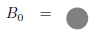
\includegraphics[width=\textwidth]{21.1}
					\caption{}
					\label{fig:21.1}
				\end{figure}\begin{figure}[H]
					\centering
					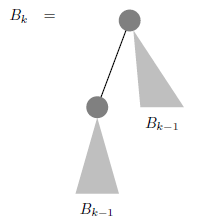
\includegraphics[width=\textwidth]{21.2}
					\caption{}
					\label{fig:21.2}
				\end{figure}
			\end{minipage} & \begin{minipage}{0.7\textwidth}
 				\begin{enumerate}
 				    \item How many nodes does $B_{k}$ have, what is its height, and how many children does its root have?
					\oldanswer{There are $2^{k}$ nodes.
					Its height is $k$.
					The root has $k$ children.}
					\item Why are they called binomial trees?
					\oldanswer{The binomial numbers represent how many nodes there are on each level.}
 				\end{enumerate}
			\end{minipage}\\
			\bottomrule
		\end{tabular}
	\end{threeparttable}\label{tab:binomial-heaps}
\end{table}

A binomial heap is a collection (linked list) of binomial trees in which each binomial tree is \textbf{heap-ordered}: each node is greater than or equal to its parent.
Also, in a binomial heap at most one instance of $B_{i}$ may occur for any $i$.

\begin{enumerate}[start=3]
    \item How many binomial trees are needed at most in the linked list of roots to make a binomial heap of $n$ nodes?
	\oldanswer{You would need $\lg n$ binomial trees at most to make a binomial heap of $n$ nodes.}
	\item See \url{https://www.cs.usfca.edu/~galles/visualization/BinomialQueue.html} to help describe how each operation is done, and its run time:
\end{enumerate}

\binomialqueueop{Make-Heap} $O(1)$, just give me a node that acts as $B_{0}$ and put the value in.
\binomialqueueop{Minimum}
Linear walk of root list: $O(\lg n)$.

\binomialqueueop{Union}

\binomialqueueop{Insert}
\oldanswer{Create a new $B_{0}$ heap and insert it at the front of the root list.
Look at the next Binomial tree in the root list, and if they have the same size, merge the 2 ``heap order'' $O(\lg n)$.}

\binomialqueueop{Extract-Min}
\oldanswer{It would take $O(\lg n)$ to find the minimum value, and then you merge the children of the max back into the root list.}

\binomialqueueop{Decrease-Key}
\oldanswer{$O(\lg n)$.
Assume we are at the node in the binomial heap.
You remove the node and, if the value of the child is smaller than the value of the root, you would switch the values and keep walking that switch up.}

\binomialqueueop{Delete}
\oldanswer{$O(\lg n)$.
Assume \_\_\_ at that node, make its value $-\infty$, call \Call{Decrease-Key}{} and then \Call{Extract-Min}{} to remove the $-\infty$.}

%</Lecture-Activity-21>

\end{document}